\section{Recurrent Neural Networks}
\label{sect:recurrent-neural-networks}
\textit{Recurrent Neural Networks} unterscheiden sich von anderen neuronalen Netzen in dem Punkt, dass sie einen (oder mehrere) Zustände speichern und verwenden können. Dabei ist ein Zustand ein berechneter Wert des vorherigen Zeitschritts. Diese Zustände können widerrum als Input genutzt werden. Somit ist eine zeitliche Zustandsspeicherung möglich.

\subsection{Sequence Learning}
\label{ssect:sequence-learning}
Sequenzen sind überall in unserem alltäglichem Leben vertreten: z.B. bei der Sequenzierung von Töne in Sprache. Bei der Spracherkennung wird der Fokus auf Wortsequenzen gelegt. 
Bei sequence learning gibt es vier generelle Probleme:
\begin{itemize}
	\item sequence prediction: Was wird das nächste Element in der Sequenz sein?
	\item sequence generation: generieren einer Sequenz (eg. Wortsequenz)
	\item sequence recognition: Ist die Sequenz legitim?
	\item sequence decision making: ??
\end{itemize}
% properly refer to the picture
\begin{figure}[h]
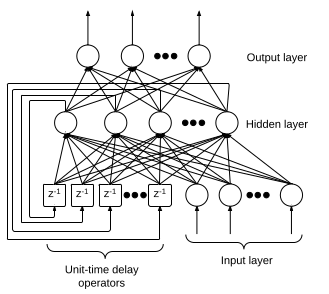
\includegraphics[scale=1.0]{rnn-example1}
\end{figure}

\subsection{Elman vs. Jordan Networks - Simple RNN}
\label{ssect:elman-vs-jordan-networks-simple-rnn}
Der Unterschied zwischen \textit{Elman} und \textit{Jordan} Netzen besteht darin, dass sie unterschiedliche Outputs zwischenspeichern und wiederverwenden. Bei Elman Netzen wird der Output des Hidden Layers als Input für den nächsten Zeitschritt verwendet. Jorden Netze auf der anderen Seite nutzen den Output des Netzes als Input für den nächsten Zeitschritt.

\subsection{Aufbau}
\label{ssect:rnn-aufbau}
% TODO: insert graphic of a rnn
\begin{itemize}
	\item Input Units $X = x_1, x_2, ..., x_n$
	\item Output Units $Y = y_1, y_2, ..., y_n$
	\item Hidden Units $H = h_1, h_2, ..., h_n$
	\item Connections between Units
\end{itemize}
Im Prinzip sehen RNN genauso aus wie NN. Jedoch sind die Verbindungen anders. Diese können nämlich zurückführen und als Input dienen. Somit lassen sich vergangene States wiederverwenden. Alternative könnte man \textit{recurrent hidden units} in den Aufbau mit aufnehmen. Diese speichern vergangene Zustände und leiten diese als Input in den darauffolgenden Zeitschritt in die entsprechenden Units.
\subsection{Training}
\label{ssect:rnn-training}
RNN werden mittels \textit{backpropagation through time} trainiert. Dies ist eine Erweiterung des ursprünglichen Backpropagation, bei der die wiederkehrenden Zustände berücksichtigt werden. Dazu wird ein RNN \textit{ausgerollt} um den zeitlichen Zusammenhang darzutellen:
\begin{figure}
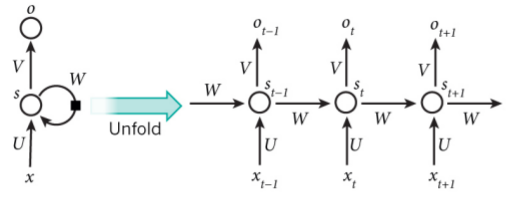
\includegraphics[scale=0.6]{unfold-example}
\end{figure}
Zu jedem Zeitpunkt nutzen wir \textit{forward pass} um die Aktivität in jedem Zeitschritt zu berechnen. Mittels \textit{backward pass} wird die Fehlerableitung zu jedem Zeitschritt berechnet.
In dem entrollten Netzwerk kommen die selben Gewichte öfters vor (shared weights), zu sehen in Bild XX. Jede Instanz eines Gewichtes muss den selben Gradienten erhalten (Einschränkung):
\begin{itemize}
	\item[1.]$w_j^{t_1} = w_j^{t_2} \Rightarrow \Delta w_j^{t_1} = \Delta w_j^{t_2}$
	\item[2.]Berechne $\frac{\partial E}{\partial w_j^{t_1}}$ und $\frac{\partial E}{\partial w_j^{t_2}}$
	\item[3.] $\Delta w_j^{t_1} = \Delta w_j^{t_2} = -\eta \left(\frac{\partial E}{\partial w_j^{t_1}} + \frac{\partial E}{\partial w_j^{t_2}}\right)$
\end{itemize}
Hierbei kann zum einen die Summe betrachtet werden, aber auch der Durchschnitt!

\subsection{Vanishing / Exploding Gradient}
\label{ssect:vanishing-exploding-gradient}


\newpage